\documentclass[conference]{IEEEtran}
\pagestyle{plain}

\usepackage{graphicx}
\graphicspath{{./imagenes/}{../imagenes/}}
\DeclareGraphicsExtensions{.pdf,.jpeg,.png}
\usepackage{changepage}
\usepackage[utf8]{inputenc}
\usepackage[T1]{fontenc}
\usepackage{microtype}
\usepackage{xcolor}
\usepackage[cmex10]{amsmath}
\usepackage{circuitikz, siunitx}
\usepackage{float}
\usepackage{array}
\usepackage{url}
\usepackage{makecell}
\usepackage{booktabs}
\usepackage{hyperref}
\def\figureautorefname{Figura}
\def\equationautorefname{Ecuación}
\usepackage{tikz}
\usepackage{pgfplots}
\pgfplotsset{compat=1.18} 
\usetikzlibrary{shapes.geometric, arrows, arrows.meta, positioning, patterns, trees}

\tikzset{
    startstop/.style={rectangle, rounded corners, minimum width=2.5cm, minimum height=1cm, text centered, draw=black, fill=gray!10},
    io/.style={trapezium, trapezium stretches=true, trapezium left angle=70, trapezium right angle=110, minimum width=2cm, minimum height=1cm, text centered, draw=black, fill=blue!10},
    process/.style={rectangle, minimum width=2.5cm, minimum height=1cm, text centered, text width=2.5cm, draw=black, fill=green!10},
    decision/.style={diamond, aspect=1.5, minimum width=2.5cm, minimum height=1cm, text centered, draw=black, fill=yellow!10},
    arrow/.style={thick,->,>=stealth},
    invarrow/.style={thick,<-,>=stealth}
}

\IEEEoverridecommandlockouts{}

\tolerance=10000
\hbadness=10000
\emergencystretch=10pt

\begin{document}

\title{Implementación y Análisis de un Conversor Analógico-Digital por Aproximaciones Sucesivas (SAR) con DAC R-2R}

\author{
    \IEEEauthorblockN{J. Pineda, M. Rodríguez y J. Salazar}
    \IEEEauthorblockA{
        \textit{Universidad de los Llanos} \\
        \textit{Villavicencio, Colombia} \\
        {\small \texttt{jspineda.ospina@unillanos.edu.co} \quad 161004610}\\
        {\small \texttt{marodriguez.payares@unillanos.edu.co} \quad 161004834}\\
        {\small \texttt{jssalazar.vargas@unillanos.edu.co} \quad 161004938}
    }
}

\IEEEaftertitletext{\vspace{-1\baselineskip}}
\maketitle

\renewcommand\abstractname{Resumen}
\begin{abstract}
En este trabajo se armó y evaluó un conversor analógico-digital SAR de 12 bits utilizando componentes discretos. La lógica de búsqueda binaria se programó en un ESP32, el cual alimenta directamente una red resistiva R-2R encargada de generar el voltaje de prueba. Para poder observar el estado de cada bit en la protoboard sin alterar los voltajes del circuito, se conectaron transistores en colector común que manejan la corriente de los LEDs de forma aislada. El ciclo de conversión se cierra con un operacional LM358P que compara la salida del DAC frente al voltaje real que se desea medir. Toda la evolución matemática del algoritmo se transmitió por puerto serial a una aplicación hecha en Python, lo que permitió graficar los saltos de la señal en tiempo real. Al probar el montaje tanto con voltajes fijos como con una onda senoidal de 100~Hz, se logró muestrear y reconstruir la señal sin problemas. Por último, el análisis de error demostró cómo ciertos factores del hardware, como la resistencia parásita en los pines del microcontrolador, le restan mucha precisión al sistema, dejando claro por qué este tipo de arquitecturas son complicadas de afinar fuera de un circuito integrado comercial.
\end{abstract}

\renewcommand\IEEEkeywordsname{Palabras clave}
\begin{IEEEkeywords}
ADC SAR, Conversión Analógica-Digital, Red R-2R, ESP32, Teorema de Nyquist, Cuantización.
\end{IEEEkeywords}

\section{Introducción}

La conversión de señales analógicas a formato digital es un proceso fundamental en los sistemas de control y medición modernos~\cite{Pavan2024}. Entre los distintos tipos de conversores, la arquitectura de aproximaciones sucesivas (SAR) destaca por ofrecer un buen balance entre velocidad, resolución y consumo de energía~\cite{Huang2025}. 

A diferencia de los conversores de rampa o los veloces ADCs tipo \textit{Flash}, el método SAR encuentra el valor del voltaje utilizando una búsqueda binaria. Esto permite que una conversión de $n$ bits se complete en exactamente $n$ ciclos de reloj. A nivel académico, construir este sistema paso a paso con componentes discretos ayuda a comprender mejor el error de cuantización y los tiempos necesarios para procesar la señal.

El objetivo de este informe es analizar el diseño y funcionamiento de un ADC SAR de 12 bits construido con un microcontrolador ESP32, una escalera resistiva R-2R y un comparador analógico. El documento detalla el cálculo de la red resistiva, el diseño de la etapa de visualización con transistores, y las pruebas experimentales realizadas. Finalmente, se analizan los errores generados por las tolerancias físicas del circuito y los pines del microcontrolador.

\section{Fundamento Teórico}

\subsection{El Conversor Digital-Analógico (DAC) tipo R-2R}
La base para que el sistema pueda efectuar iteraciones comparativas reside en la capacidad de sintetizar voltajes analógicos precisos a partir de suposiciones digitales discretas. Para ello se recurrió a un DAC de topología R-2R. La elegancia matemática de este circuito radica en el empleo de únicamente dos valores resistivos (proporción 1:2), solventando el problema de los DAC de resistencias ponderadas que exigen componentes de altísima impedancia e inalcanzable precisión para los bits de menor peso estadístico.

\begin{figure}[htbp]
    \centering
    \resizebox{\columnwidth}{!}{
    \begin{circuitikz}[scale=0.85, transform shape, line width=0.8pt]
        % LSB node y terminacion
        \draw (0,0) node[ground]{} to[R, l=$2R$] (0,2);
        \draw (2,0) node[below]{$D_0$ (LSB)} to[R, l=$2R$, o-*] (2,2);
        \draw (0,2) -- (2,2);
        \draw (2,2) to[R, l=$R$] (4.5,2);
        
        % D1 Branch
        \draw (4.5,0) node[below]{$D_1$} to[R, l=$2R$, o-*] (4.5,2);
        \draw (4.5,2) to[R, l=$R$] (7,2);
        
        % Dots
        \node at (8,2) {\Large $\dots$};
        
        % D10 Branch
        \draw (9,2) to[R, l=$R$] (11.5,2);
        \draw (9,0) node[below]{$D_{10}$} to[R, l=$2R$, o-*] (9,2);
        
        % D11 Branch
        \draw (11.5,0) node[below]{$D_{11}$ (MSB)} to[R, l=$2R$, o-*] (11.5,2);
        \draw (11.5,2) to[short, -o] (13,2) node[right]{$V_{\text{DAC}}$};
    \end{circuitikz}
    }
    \caption{Esquema eléctrico de la red DAC tipo R-2R analizada. Las entradas digitales $D_0 \dots D_{11}$ inyectan tensión y corriente ponderadas secuencialmente en potencias de dos a lo largo de la escalera hacia el nodo colector $V_{\text{DAC}}$.}\label{fig:circuito_r2r}
\end{figure}

El funcionamiento se deduce matemáticamente al iterar el teorema de Thévenin. Observando desde cualquier nodo interno hacia la izquierda (hacia el LSB), la impedancia equivalente siempre es $R$. Por ende, cada nodo divide la corriente inyectada por la rama digital correspondiente exactamente a la mitad, ponderando de forma binaria natural la contribución de cada pin $D_i$ sobre el voltaje total de salida $V_{\text{DAC}}$. Para el presente montaje, se emplearon resistores de $R = 1\text{ k}\Omega$ y $2R = 2\text{ k}\Omega$.

\subsection{El Algoritmo de Aproximaciones Sucesivas (SAR)}
El principio operativo del algoritmo SAR es análogo a una búsqueda en árbol dicotómico. El microcontrolador inicia el ciclo asumiendo que el valor desconocido se halla exactamente en el centro del rango de medición. Para ello, enciende exclusivamente el bit más significativo (MSB = 1) y apaga el resto, generando un nivel de prueba de $V_{\text{ref}}/2$ en el nodo de convergencia del DAC. 

\begin{figure}[htbp]
    \centering
    \resizebox{\columnwidth}{!}{
    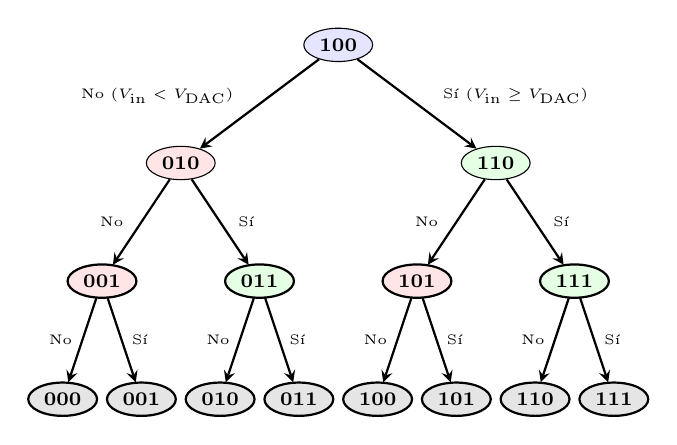
\begin{tikzpicture}[
        level 1/.style={sibling distance=4cm, level distance=1.5cm},
        level 2/.style={sibling distance=2cm, level distance=1.5cm},
        level 3/.style={sibling distance=1cm, level distance=1.5cm},
        edge from parent/.style={draw, ->, >=stealth, thick},
        node/.style={ellipse, draw, fill=blue!10, text centered, inner sep=2pt, font=\scriptsize\bfseries}
    ]
        \node[node] {100}
            child {node[node, fill=red!10] {010}
                child {node[node, fill=red!10] {001}
                    child {node[node, fill=gray!20] {000} edge from parent node[left, font=\tiny] {No}}
                    child {node[node, fill=gray!20] {001} edge from parent node[right, font=\tiny] {Sí}}
                    edge from parent node[left, font=\tiny, xshift=-0.1cm] {No}
                }
                child {node[node, fill=green!10] {011}
                    child {node[node, fill=gray!20] {010} edge from parent node[left, font=\tiny] {No}}
                    child {node[node, fill=gray!20] {011} edge from parent node[right, font=\tiny] {Sí}}
                    edge from parent node[right, font=\tiny, xshift=0.1cm] {Sí}
                }
                edge from parent node[left, font=\tiny, xshift=-0.2cm, yshift=0.1cm] {No ($V_{\text{in}} < V_{\text{DAC}}$)}
            }
            child {node[node, fill=green!10] {110}
                child {node[node, fill=red!10] {101}
                    child {node[node, fill=gray!20] {100} edge from parent node[left, font=\tiny] {No}}
                    child {node[node, fill=gray!20] {101} edge from parent node[right, font=\tiny] {Sí}}
                    edge from parent node[left, font=\tiny, xshift=-0.1cm] {No}
                }
                child {node[node, fill=green!10] {111}
                    child {node[node, fill=gray!20] {110} edge from parent node[left, font=\tiny] {No}}
                    child {node[node, fill=gray!20] {111} edge from parent node[right, font=\tiny] {Sí}}
                    edge from parent node[right, font=\tiny, xshift=0.1cm] {Sí}
                }
                edge from parent node[right, font=\tiny, xshift=0.2cm, yshift=0.1cm] {Sí ($V_{\text{in}} \ge V_{\text{DAC}}$)}
            };
    \end{tikzpicture}
    }
    \caption{Árbol de búsqueda binaria para un ADC de 3 bits.}\label{fig:arbol_sar}
\end{figure}

El amplificador operacional evalúa esta hipótesis. Si el voltaje del DAC supera al de entrada, el comparador emite un cero, descartando el bit. Si la entrada es mayor, el bit se mantiene. El proceso desciende secuencialmente hasta el bit menos significativo (LSB).

\section{Metodología e Implementación de Hardware}

El circuito se controló con un microcontrolador ESP32 programado en C++ (PlatformIO), utilizando una comunicación serial a $4.608\text{ Mbaudios}$ para reducir los tiempos de transmisión (\autoref{fig:diagrama_completo}). Se emplearon doce pines GPIO (del $D_{11}$ al $D_0$) para alimentar la escalera resistiva R-2R.

\begin{figure}[htbp]
    \centering
    \resizebox{\columnwidth}{!}{
    \begin{circuitikz}[scale=0.9, transform shape, line width=0.8pt]
        % ESP32 block
        \draw[thick] (-1,0) rectangle (2,5);
        \node at (0.5,2.5) {\textbf{ESP32}};
        \node[left] at (2, 4.5) {$D_i$};
        \node[right] at (-1, 1) {Pin 34 (In)};

        % Serial Pin at North
        \draw (0.5, 5) to[short, -o] (0.5, 5.8) node[above, font=\small] {Serial};

        % R-2R Representative Block
        \draw (2, 3.5) |- (4, 4.5);
        \draw (4, 4.5) -- (4, 6.0);
        \draw (4, 6.0) to[R, l=$2R$] (4, 7.5);
        \draw (4, 7.5) |- (4, 8.5) to[R, l=$R$] (7.5, 8.5);
        \draw (7.5, 8.5) -- (11.3, 8.5) node[pos=0.5, above]{$V_{\text{DAC}}$};
        \draw (2, 8.5) to[R, l=$2R$] (2, 6.5) node[ground]{};
        \draw[dashed] (2, 8.5) -- (4, 8.5);

        % Transistor stage (Example for one pin)
        \draw (4, 4.5) to[R, l=$10\text{k}\Omega$] (6, 4.5);
        \draw (7, 4.5) node[npn, tr circle] (npn) {};
        \draw (6, 4.5) -- (npn.B);
        \draw (npn.C) -- (7, 5.5) node[vcc]{$+5\text{V}$};
        \draw (npn.E) to[R, l=$330\Omega$] (7, 2.5);
        \draw (7, 2.5) to[leD, l=LED] (7, 1) node[ground]{};
        
        % Label for the 12 modules
        \draw[dashed, color=gray, thick] (3, -0.5) rectangle (8.7, 9.5);
        \node[font=\footnotesize] at (6, 0) {$\times 12$ Módulos};

        % Comparator
        \draw (12.5, 8.0) node[op amp] (opamp) {}; 
        \draw (11.3, 8.5) -- (opamp.-);
        
        % Power of Comparator
        \draw (opamp.up) -- ++(0,0.5) node[vcc]{$+8\text{V}$};
        \draw (opamp.down) -- ++(0,-0.5) node[ground]{};
        
        % Potentiometer
        \draw (10.5, 6.5) to[pR, n=pot] (10.5, 4.5);
        \draw (10.5, 6.5) node[vcc]{$+3.3\text{V}$};
        \draw (10.5, 4.5) node[ground]{};
        \draw (pot.wiper) |- (opamp.+);
        \node[left, align=right] at (10.2, 5.5) {$V_{\text{ref}}$};
        
        % Trimmer
        \draw (opamp.out) -- (14.5, 8.0);
        \draw (14.5, 8.0) to[pR, n=trim] (14.5, 5.0);
        \draw (14.5, 5.0) node[ground]{};
        
        % Return to ESP32 Pin 34
        \draw (trim.wiper) -- (15.5, 6.5) -- (15.5, -1) -- (-1.5, -1) -- (-1.5, 1) -- (-1, 1);
        \end{circuitikz}
    }
    \caption{Diagrama esquemático del sistema implementado. Se observa la red R-2R, una etapa de visualización de alta impedancia (colector común) y el comparador analógico con protección de voltaje para la ESP32.}
    \label{fig:diagrama_completo}
\end{figure}


\subsection{Acoplamiento de Impedancias y Visualización}
Para ver el estado binario en la protoboard, conectar los LEDs directamente a la escalera R-2R habría demandado demasiada corriente, alterando los voltajes precisos del DAC analógico. 

Para solucionar esto, se implementó una etapa con transistores NPN configurados en \textit{colector común}. El colector se conectó a los $5\text{V}$ de la fuente, mientras que la base se unió al pin del ESP32 mediante una resistencia de $10\text{ k}\Omega$. El emisor encendía el LED rojo a través de un resistor limitador de $330\text{ }\Omega$. Esta configuración garantiza una impedancia de entrada alta, proveyendo a los LEDs la corriente necesaria sin desestabilizar la red R-2R.

\subsection{Lazo de Comparación Analógica}
La lectura del voltaje la realiza un amplificador operacional LM358P, alimentado con $8\text{V}$ y GND. La entrada no inversora (+) se conectó a un potenciómetro (señal a medir) alimentado a $3.3\text{V}$, mientras que la inversora (-) recibe el voltaje dinámico generado por el DAC. 

Dado que el operacional en estado alto entrega cerca de $6.5\text{V}$ y el pin del ESP32 solo soporta $3.3\text{V}$, se utilizó un trimmer como divisor de voltaje para atenuar la salida del comparador hasta niveles lógicos seguros.

\subsection{Instrumentación Virtual (GUI en Python)}
En su código interno, el microcontrolador efectúa el algoritmo SAR enmascarando los pines GPIO. En las pruebas iníciales se incluyó un retardo programado de $1\text{ segundo}$ para visualizar los pasos, interrogando luego el estado lógico devuelto por el comparador (pin 34). 

\begin{figure}[htbp]
    \centering
    \resizebox{\columnwidth}{!}{
    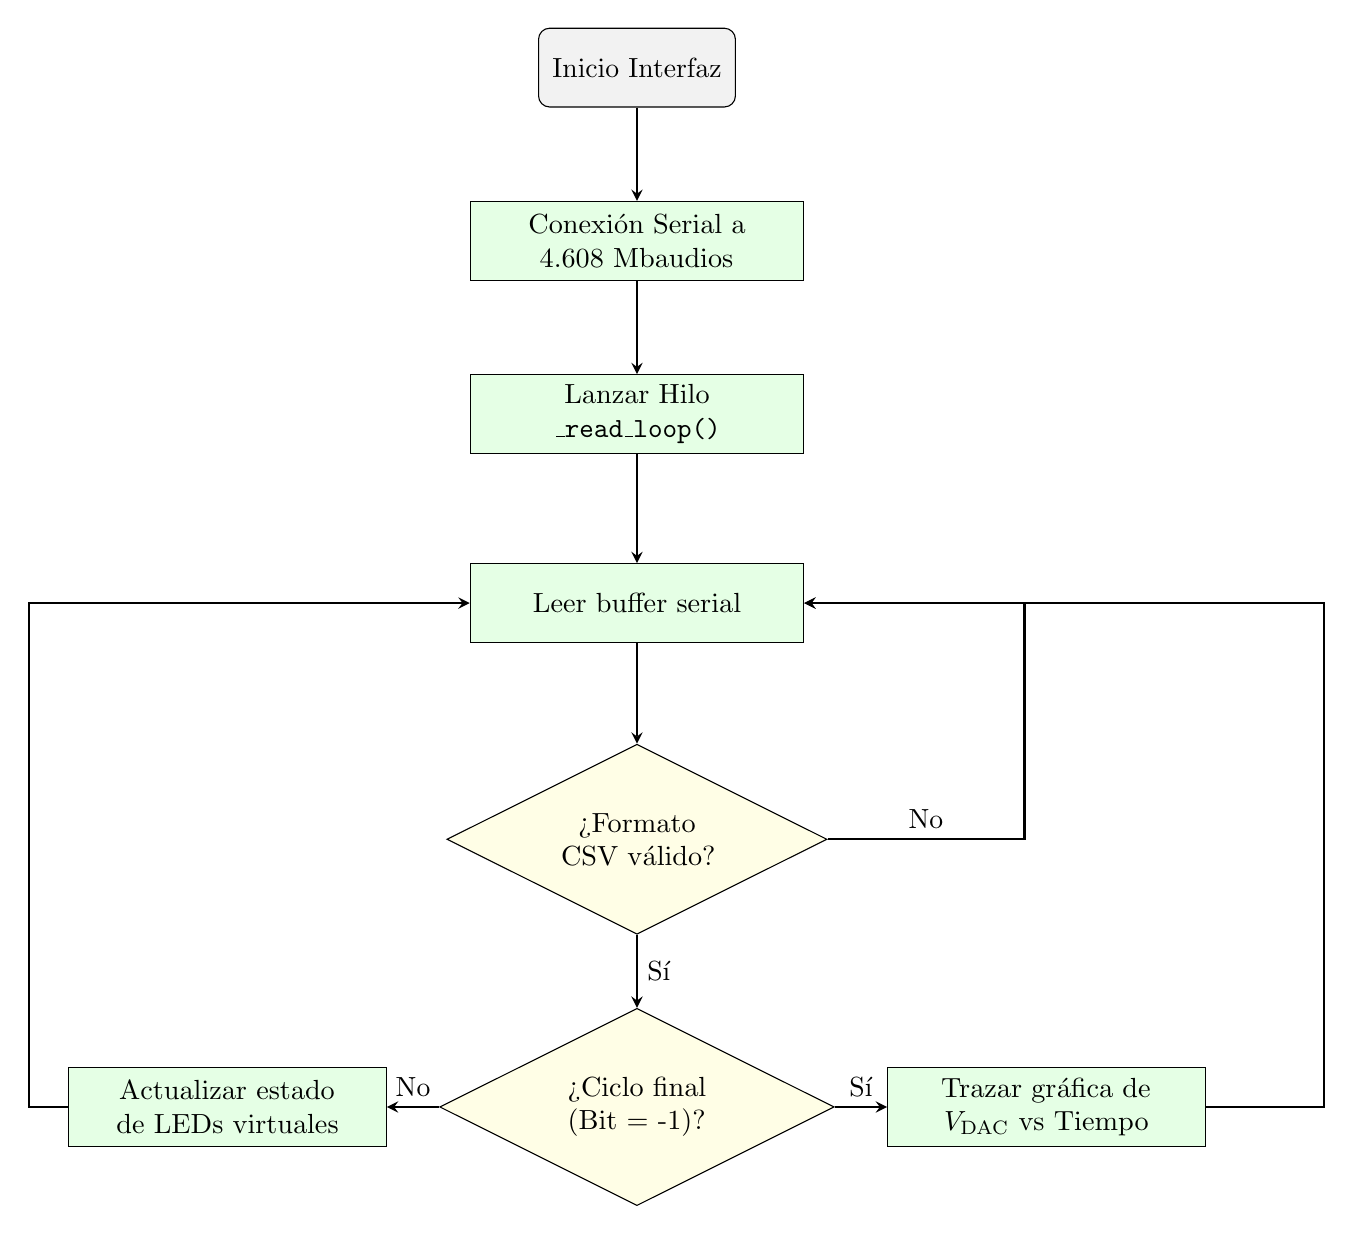
\begin{tikzpicture}[node distance=2.2cm]
        \node (start) [startstop] {Inicio Interfaz};
        \node (connect) [process, below of=start, text width=4cm] {Conexión Serial a 4.608 Mbaudios};
        \node (thread) [process, below of=connect, text width=4cm] {Lanzar Hilo \texttt{\_read\_loop()}};
        
        \node (loop) [process, below of=thread, yshift=-0.2cm, text width=4cm] {Leer buffer serial};
        \node (valid) [decision, below of=loop, yshift=-0.8cm, aspect=2, text width=2.8cm] {¿Formato CSV válido?};
        
        \node (checkbit) [decision, below of=valid, yshift=-1.2cm, aspect=2, text width=2.8cm] {¿Ciclo final \\ (Bit = -1)?};
        
        \node (updatetest) [process, left of=checkbit, xshift=-3cm, text width=3.8cm] {Actualizar estado de LEDs virtuales};
        \node (updateui) [process, right of=checkbit, xshift=3cm, text width=3.8cm] {Trazar gráfica de $V_{\text{DAC}}$ vs Tiempo};
        
        \draw [arrow] (start) -- (connect);
        \draw [arrow] (connect) -- (thread);
        \draw [arrow] (thread) -- (loop);
        \draw [arrow] (loop) -- (valid);
        
        \draw [arrow] (valid.east) -- node[midway, above] {No} ++(2.5,0) |- (loop.east);
        \draw [arrow] (valid.south) -- node[midway, right] {Sí} (checkbit.north);
        
        \draw [arrow] (checkbit.west) -- node[midway, above] {No} (updatetest.east);
        \draw [arrow] (checkbit.east) -- node[midway, above] {Sí} (updateui.west);
        
        \draw [arrow] (updatetest.west) -- ++(-0.5,0) |- (loop.west);
        \draw [arrow] (updateui.east) -- ++(1.5,0) |- (loop.east);
    \end{tikzpicture}
    }
    \caption{Diagrama de flujo de la interfaz en Python. Leer los datos por puerto serial en un hilo secundario (\textit{thread}) evita interbloqueos y evita que la aplicación principal se congele.}\label{fig:flujo_python}
\end{figure}

Todos los datos de las iteraciones se enviaron por serial a la computadora para procesarlos en una aplicación de escritorio diseñada en Python (\autoref{fig:flujo_python}). Los paquetes de datos se transmitieron en formato CSV (texto separado por comas), incluyendo el índice del bit evaluado, el voltaje de prueba y el tiempo. El software extrae estos valores para actualizar los indicadores virtuales y dibujar la gráfica de convergencia usando las librerías \texttt{Tkinter} y \texttt{Matplotlib}.

\section{Resultados y Análisis de Error}

\subsection{Validaci\'on del Sistema mediante Simulaci\'on}

De manera preliminar a los ensayos f\'isicos, el comportamiento de la arquitectura dise\~nada se evalu\'o mediante la plataforma \textit{Simulink} de MATLAB~\cite{simulink_mathworks}. Dicha simulaci\'on hizo posible aislar anomal\'ias y verificar la convergencia rigurosa del mecanismo de b\'usqueda binaria del SAR de 12 bits dentro de un ecosistema exento de tolerancias f\'isicas. El esquema del modelo (\autoref{fig:simulacion_circuito}) hibrida elementos propios de la biblioteca \textit{Simscape} ---para la l\'inea anal\'ogica de resistencias, fuentes controladas y el comparador--- con una funci\'on discreta de MATLAB encargada de emular la ejecuci\'on l\'ogica y secuencial originada en el ESP32.

\begin{figure}[htbp]
    \centering
    \includegraphics[width=\columnwidth]{circuito_simulacion.png}
    \caption{Estructura del modelo mixto elaborado en \textit{Simulink}. Se puede observar la integraci\'on de la escalera resistiva, el m\'odulo central del microcontrolador y el lazo de retroalimentaci\'on del comparador.}
    \label{fig:simulacion_circuito}
\end{figure}

El perfil arrojado por el osciloscopio virtual (\autoref{fig:simulacion_plot}) ilustra emp\'iricamente la formaci\'on de la aproximaci\'on sobre una se\~nal senoidal continua. En cada etapa de muestreo, el conversor arranca analizando el bit de mayor peso (el MSB, dividiendo a la mitad la tensi\'on de referencia) para luego refinar el valor a trav\'es de los niveles inferiores iterativamente. Este acercamiento escalonado demuestra un rastreo sumamente eficiente de la entrada $V_{in}$, consiguiendo acorralar la onda base en tan solo doce pasos de resoluci\'on.

\begin{figure}[htbp]
    \centering
    \includegraphics[width=\columnwidth]{simulacion.png}
    \caption{Din\'amica temporal del proceso de aproximaciones sucesivas. La se\~nal $V_{DAC}$ arranca su exploraci\'on desde el MSB, reduciendo el rango de certidumbre progresivamente hasta enclavar el voltaje anal\'ogico.}
    \label{fig:simulacion_plot}
\end{figure}

A nivel algor\'itmico, estos resultados garantizan que ---eliminando imperfecciones del hardware como fluctuaciones de temperatura o resistencias par\'asitas--- el sondeo dicot\'omico aproxima de manera ideal el l\'imite de cuantizaci\'on.


\subsection{Cálculo de Resolución e Incertidumbre}
Para el microcontrolador utilizado, el nivel lógico alto que alimenta la red R-2R es $V_{\text{ref}} = 3.3\text{ V}$. Al trabajar con 12 bits ($2^{12} - 1 = 4095$ niveles), el valor de cada paso de cuantización (LSB) es:

\begin{equation}
    V_{\text{LSB}} = \frac{3.3\text{ V}}{4095} 
\end{equation}
\approx 805.86\,\mu\text{V}
En un sistema ideal, el ruido de cuantización máximo sería de $\pm 0.5 \text{ LSB} \approx 402.9\,\mu\text{V}$~\cite{Fukazawa2023, Li2023}. Sin embargo, los componentes físicos introducen errores mayores en el circuito real:
\begin{enumerate}
    \item \textbf{Impedancia de los pines GPIO (Error Dinámico):} Aunque la red R-2R se calibró con potenciómetros de precisión para corregir los valores de las resistencias, el propio ESP32 introduce un error. Los transistores internos que generan el nivel alto en los pines GPIO tienen una resistencia de encendido ($R_{DS(on)}$) de entre $30\,\Omega$ y $40\,\Omega$~\cite{esp32_datasheet}. Esta resistencia se suma a la rama de $2\text{ k}\Omega$. Para el bit más significativo (MSB), asumiendo un $R_{DS(on)}$ de $30\,\Omega$, el error sobre el voltaje ideal de $1.65\text{ V}$ se calcula en la \autoref{eq:error_msb}:
    \begin{equation}
        \Delta V_{\text{MSB}} \approx 1.65\text{ V} \times 0.015 = 24.75\text{ mV}
        \label{eq:error_msb}
    \end{equation}
    Este error es mucho mayor que el LSB. Dividiendo este valor entre el LSB, obtenemos el error equivalente (\autoref{eq:error_msb_lsb}):
    \begin{equation}
        E_{\text{MSB}} = \frac{\Delta V_{\text{MSB}}}{V_{\text{LSB}}} = \frac{24.75\text{ mV}}{805.86\,\mu\text{V}} \approx 30.7 \text{ LSB}
        \label{eq:error_msb_lsb}
    \end{equation}
    Este error de casi $31\text{ LSBs}$ afecta fuertemente la linealidad diferencial (DNL) del convertidor~\cite{Centurelli2022}.
    \item \textbf{Voltaje de Offset del LM358P:} Según la hoja de datos de Texas Instruments~\cite{lm358_datasheet}, el LM358 tiene un voltaje de offset de entrada nominal de $2\text{ mV}$ (máximo $7\text{ mV}$). Este voltaje se traduce en un error constante (\autoref{eq:error_offset}):
    \begin{equation}
        E_{\text{offset}} = \frac{V_{\text{offset}}}{V_{\text{LSB}}} = \frac{2\text{ mV}}{805.86\,\mu\text{V}} \approx 2.48 \text{ LSB}
        \label{eq:error_offset}
    \end{equation}
    En el peor de los casos, este offset puede llegar hasta $8.5 \text{ LSBs}$, afectando la comparación.
\end{enumerate}

Debido a estos factores, aunque se usaron potenciómetros de precisión para ajustar la red, las limitaciones del microcontrolador y del operacional reducen la resolución efectiva del ADC a unos $7\text{ bits}$ reales~\cite{Huang2025, Shibata2023}.

\subsection{Validación con Voltaje Estático (DC)}
En la primera prueba, se utilizó el potenciómetro para introducir un voltaje DC constante. El proceso de búsqueda binaria se observó tanto en los LEDs del circuito (\autoref{fig:prueba_dc}) como en la interfaz gráfica de Python (\autoref{fig:prueba_dc_graf} y \autoref{fig:gui_runtime}).

\begin{figure}[htbp]
    \centering
    \resizebox{\columnwidth}{!}{
        \includegraphics{montaje.png}
    }
    \caption{Fotografía del circuito ensamblado. \textbf{Azul}: Señal de entrada. \textbf{Amarillo}: Etapa de LEDs (visualización). \textbf{Verde}: Red DAC R-2R. \textbf{Rojo}: Comparador LM358P. \textbf{Blanco}: ESP32.}\label{fig:prueba_dc}
\end{figure}

\begin{figure}[htbp]
    \centering
    \resizebox{\columnwidth}{!}{
        \includegraphics{DC.PNG}
    }
    \caption{Gráfica de convergencia en DC. Se observan los saltos grandes iniciales y cómo el voltaje se afina en los últimos bits.}\label{fig:prueba_dc_graf}
\end{figure}

\begin{figure}[htbp]
    \centering
    \resizebox{\columnwidth}{!}{
        \includegraphics{GUI.png}
    }
    \caption{Interfaz en Python mostrando los LEDs virtuales y el valor final convertido.}\label{fig:gui_runtime}
\end{figure}

El sistema funcionó según lo esperado: inicia probando la mitad del voltaje de referencia y luego ajusta el valor bit a bit hasta acercarse a la tensión de entrada.

\subsection{Comportamiento Dinámico (AC)}
Para evaluar el sistema con señales variables, se conectó un generador de señales inyectando una onda senoidal de $100\text{ Hz}$ (\autoref{fig:interfaz_senoidal}). 

\begin{figure}[htbp]
    \centering
    \resizebox{\columnwidth}{!}{
        \includegraphics{AC.PNG}
    }
    \caption{Señal senoidal de 100 Hz reconstruida en la interfaz gráfica.}\label{fig:interfaz_senoidal}
\end{figure}

En la prueba de DC, el tiempo entre cada bit (\texttt{delayBetweenBits}) fue de $1\text{ segundo}$ para poder ver los LEDs encenderse. Para capturar la señal AC, este retardo se redujo a $100\,\mu\text{s}$ por bit.

Con este nuevo retardo, un ciclo completo de conversión de 12 bits toma unos $1.2\text{ ms}$, lo que equivale a una frecuencia de muestreo de $\sim 833\text{ Hz}$. Esta velocidad es más que suficiente para cumplir el Teorema de Nyquist-Shannon ($f_s > 2f_{\text{max}}$) y muestrear la señal de $100\text{ Hz}$. La gráfica en Python mostró una onda senoidal bien definida, demostrando que el ESP32 y el comparador operaron lo suficientemente rápido para realizar la conversión dinámica sin deformar la señal.

\subsection{Análisis de la Arquitectura}
Construir un ADC SAR con componentes discretos tiene ventajas y desventajas. Entre sus \textbf{ventajas}, destaca su valor didáctico, ya que permite ver cómo funciona internamente un convertidor que normalmente está oculto en un chip. Además, al usar código y pines digitales, el tiempo de conversión es siempre constante (exactamente 12 iteraciones), lo cual es más rápido que otros métodos simples como el ADC de rampa~\cite{Pavan2024}.

Entre sus \textbf{desventajas}, se encuentra la dificultad para lograr alta precisión. El diseño es muy sensible a las tolerancias de las resistencias y a la resistencia interna de los pines del microcontrolador ($R_{DS(on)}$). Estos pequeños errores se acumulan y afectan los bits menos significativos. Además, el circuito requiere muchas resistencias (24 en total) y ocupa 12 pines del ESP32, lo que lo hace muy grande e ineficiente en términos de espacio.

\section{Conclusiones}

El diseño e implementación de este circuito ADC SAR combinando un ESP32, una red R-2R y un comparador resultó ser una excelente herramienta para entender en la práctica el proceso de cuantización analógico-digital~\cite{Mittal2023, Shtendel2023}. Sin embargo, los cálculos de error demostraron que construir un ADC de 12 bits con componentes discretos es un desafío considerable. A pesar de calibrar la red resistiva con potenciómetros, la resistencia interna de los pines del ESP32 generó un error dinámico de casi $31\text{ LSBs}$ (Ecuaciones \autoref{eq:error_msb} y \autoref{eq:error_msb_lsb}). Sumando a esto el voltaje de offset del operacional, la resolución útil del sistema se reduce en la práctica a unos $7\text{ bits}$.

En cuanto al análisis dinámico, el sistema demostró ser lo suficientemente rápido al digitalizar una señal AC de $100\text{ Hz}$. Al reducir el retardo del código, se logró una frecuencia de muestreo de $\sim 833\text{ Hz}$, lo que cumplió exitosamente con el teorema de Nyquist-Shannon~\cite{Lesnikov2022, Wang2022} y permitió observar una reconstrucción senoidal limpia en la interfaz de Python. Esto valida el diseño del convertidor para aplicaciones de baja frecuencia.

\bibliographystyle{IEEEtran}
\bibliography{IEEEabrv,biblio_traps_dynamics}
\end{document}
